\documentclass{article}

\usepackage{graphicx}
\usepackage{amsmath}
\usepackage{float}
\usepackage{hyperref}


%%
\author{Francesco Angelo Fabiano Antonacci}
\date{\today}
\title{Relazione Natalizia}
%%


\begin{document}
\maketitle


%%%%%%%%%%%%%%%%%%%%%%%%%%%%%%%%%%%%%%%%%%%%
\section{Ricostruzione numerica di forme d'onda}
ricostruzione numerica forme d'onda quadre e triangolari, 
con studio (qualitativo o quantitativo, dipende da quanto siete bravi!) 
dei risultati in funzione del numero di iterazioni (troncamento della serie)
 e del campionamento (numero di punti/numero di periodi degli array);
\subsection{Quadra}
\subsection{Triangolare}
\subsection{Pinna di squalo}
ricostruzione numerica della forma d'onda a pinna di squalo in uscita da integratore, 
con forma quadra in ingresso, in funzione della frequenza 
(per una data frequenza di taglio);

%%%%%%%%%%%%%%%%%%%%%%%%%%%%%%%%%%%%%%%%%%
\section{Simulazioni}
\subsection{Pinne di squalo}
\subsubsection{Onda quadra}
\subsubsection{Onda triangolare}

simulazione numerica dei segnali a pinna di squalo acquisiti da Arduino:
 potete aggiustare ampiezza, offset, fase a mano, oppure provare un best-fit 
 (più difficile tecnicamente); il risultato deve essere convincente!
\subsection{Guadagno e frequenze}
\subsubsection{Onda quadra}
\subsubsection{Onda triangolare}

Simulazione numerica dei grafici guadagno vs frequenza costruiti in laboratorio 
per un integratore con forma d'onda quadra in ingresso:
 cercate di contestualizzare per bene!


\subsection{Derivatore}

facoltativamente potete ripetere i punti 2 e 3 anche supponendo di impiegare
 un derivatore, con forma d'onda in ingresso a vostra scelta: 
 qui, per motivi che spero vi siano ovvi, non dovreste avere dati sperimentali;


\subsection{Forma d'onda quadra a bassa frequenza}
facoltativamente potete ricostruire una forma d'onda quadra di "bassa frequenza"
 osservata con l'oscilloscopio in accoppiamento AC (ricordate? la distorsione...);



\subsection{Forma d'onda quadra con duty cycle variabile}
sempre facoltativamente (ma importantemente, 
poiché vedremo sperimentalmente questo aspetto al ritorno dalle vacanze) 
potete ricostruire una forma d'onda quadra con duty cycle variabile, 
ovvero treno di impulsi, e vedere l'effetto quando essa viene inviata 
a un filtro passa-basso (con frequenza di taglio minore della frequenza
 dell'onda quadra). Vedete di capirci qualcosa!


\begin{figure}[h!]
    \centering
    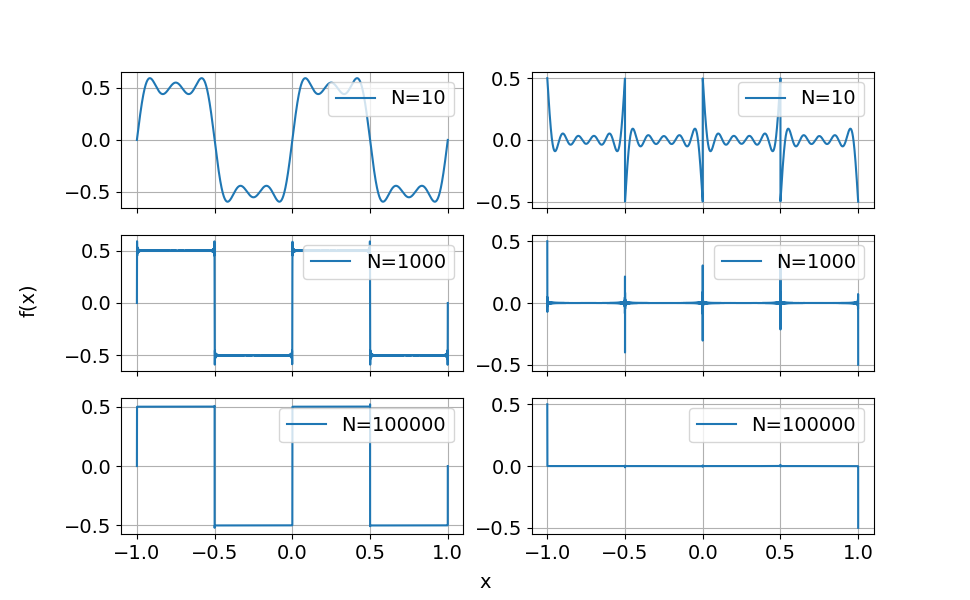
\includegraphics[width=1.2\textwidth]{fousquarewave.png} % Replace with your image name
    \caption{}
    \label{fig:example}
\end{figure}

\begin{figure}[h!]
    \centering
    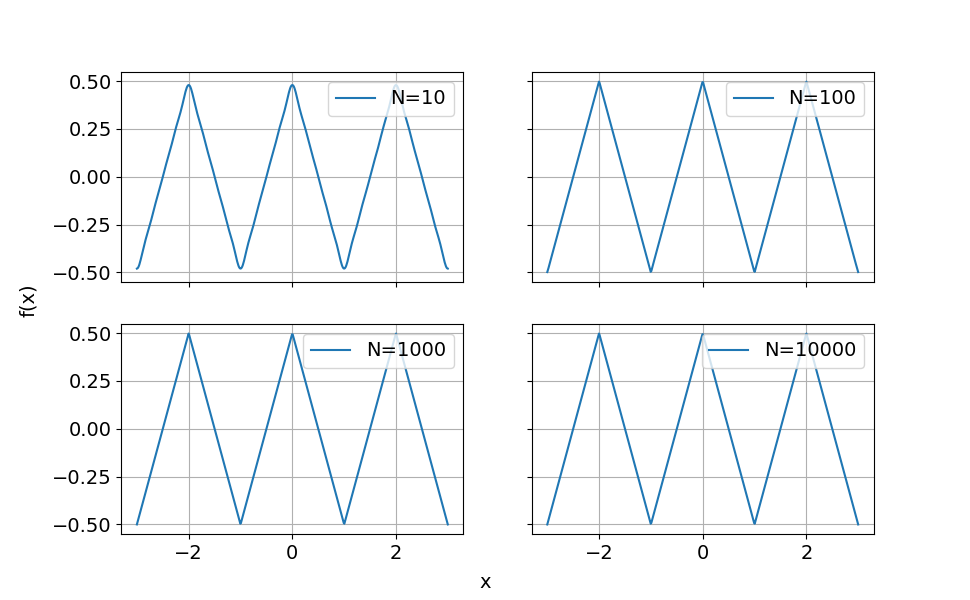
\includegraphics[width=1.2\textwidth]{foutriawave.png} % Replace with your image name
    \caption{}
    \label{fig:example}
\end{figure}

\end{document}